\documentclass[twoside]{book}

% Packages required by doxygen
\usepackage{fixltx2e}
\usepackage{calc}
\usepackage{doxygen}
\usepackage[export]{adjustbox} % also loads graphicx
\usepackage{graphicx}
\usepackage[utf8]{inputenc}
\usepackage{makeidx}
\usepackage{multicol}
\usepackage{multirow}
\PassOptionsToPackage{warn}{textcomp}
\usepackage{textcomp}
\usepackage[nointegrals]{wasysym}
\usepackage[table]{xcolor}

% Font selection
\usepackage[T1]{fontenc}
\usepackage[scaled=.90]{helvet}
\usepackage{courier}
\usepackage{amssymb}
\usepackage{sectsty}
\renewcommand{\familydefault}{\sfdefault}
\allsectionsfont{%
  \fontseries{bc}\selectfont%
  \color{darkgray}%
}
\renewcommand{\DoxyLabelFont}{%
  \fontseries{bc}\selectfont%
  \color{darkgray}%
}
\newcommand{\+}{\discretionary{\mbox{\scriptsize$\hookleftarrow$}}{}{}}

% Page & text layout
\usepackage{geometry}
\geometry{%
  a4paper,%
  top=2.5cm,%
  bottom=2.5cm,%
  left=2.5cm,%
  right=2.5cm%
}
\tolerance=750
\hfuzz=15pt
\hbadness=750
\setlength{\emergencystretch}{15pt}
\setlength{\parindent}{0cm}
\setlength{\parskip}{3ex plus 2ex minus 2ex}
\makeatletter
\renewcommand{\paragraph}{%
  \@startsection{paragraph}{4}{0ex}{-1.0ex}{1.0ex}{%
    \normalfont\normalsize\bfseries\SS@parafont%
  }%
}
\renewcommand{\subparagraph}{%
  \@startsection{subparagraph}{5}{0ex}{-1.0ex}{1.0ex}{%
    \normalfont\normalsize\bfseries\SS@subparafont%
  }%
}
\makeatother

% Headers & footers
\usepackage{fancyhdr}
\pagestyle{fancyplain}
\fancyhead[LE]{\fancyplain{}{\bfseries\thepage}}
\fancyhead[CE]{\fancyplain{}{}}
\fancyhead[RE]{\fancyplain{}{\bfseries\leftmark}}
\fancyhead[LO]{\fancyplain{}{\bfseries\rightmark}}
\fancyhead[CO]{\fancyplain{}{}}
\fancyhead[RO]{\fancyplain{}{\bfseries\thepage}}
\fancyfoot[LE]{\fancyplain{}{}}
\fancyfoot[CE]{\fancyplain{}{}}
\fancyfoot[RE]{\fancyplain{}{\bfseries\scriptsize Generated by Doxygen }}
\fancyfoot[LO]{\fancyplain{}{\bfseries\scriptsize Generated by Doxygen }}
\fancyfoot[CO]{\fancyplain{}{}}
\fancyfoot[RO]{\fancyplain{}{}}
\renewcommand{\footrulewidth}{0.4pt}
\renewcommand{\chaptermark}[1]{%
  \markboth{#1}{}%
}
\renewcommand{\sectionmark}[1]{%
  \markright{\thesection\ #1}%
}

% Indices & bibliography
\usepackage{natbib}
\usepackage[titles]{tocloft}
\setcounter{tocdepth}{3}
\setcounter{secnumdepth}{5}
\makeindex

% Hyperlinks (required, but should be loaded last)
\usepackage{ifpdf}
\ifpdf
  \usepackage[pdftex,pagebackref=true]{hyperref}
\else
  \usepackage[ps2pdf,pagebackref=true]{hyperref}
\fi
\hypersetup{%
  colorlinks=true,%
  linkcolor=blue,%
  citecolor=blue,%
  unicode%
}

% Custom commands
\newcommand{\clearemptydoublepage}{%
  \newpage{\pagestyle{empty}\cleardoublepage}%
}

\usepackage{caption}
\captionsetup{labelsep=space,justification=centering,font={bf},singlelinecheck=off,skip=4pt,position=top}

%===== C O N T E N T S =====

\begin{document}

% Titlepage & ToC
\hypersetup{pageanchor=false,
             bookmarksnumbered=true,
             pdfencoding=unicode
            }
\pagenumbering{roman}
\begin{titlepage}
\vspace*{7cm}
\begin{center}%
{\Large My Project }\\
\vspace*{1cm}
{\large Generated by Doxygen 1.8.11}\\
\end{center}
\end{titlepage}
\clearemptydoublepage
\tableofcontents
\clearemptydoublepage
\pagenumbering{arabic}
\hypersetup{pageanchor=true}

%--- Begin generated contents ---
\chapter{Hierarchical Index}
\section{Class Hierarchy}
This inheritance list is sorted roughly, but not completely, alphabetically\+:\begin{DoxyCompactList}
\item Pile\+Entiers\begin{DoxyCompactList}
\item \contentsline{section}{Alveoles\+Libres}{\pageref{classAlveolesLibres}}{}
\end{DoxyCompactList}
\item Q\+Widget\begin{DoxyCompactList}
\item \contentsline{section}{Alveoles\+Widget}{\pageref{classAlveolesWidget}}{}
\end{DoxyCompactList}
\end{DoxyCompactList}

\chapter{Class Index}
\section{Class List}
Here are the classes, structs, unions and interfaces with brief descriptions\+:\begin{DoxyCompactList}
\item\contentsline{section}{\hyperlink{classAlveolesLibres}{Alveoles\+Libres} }{\pageref{classAlveolesLibres}}{}
\item\contentsline{section}{\hyperlink{classAlveolesWidget}{Alveoles\+Widget} }{\pageref{classAlveolesWidget}}{}
\end{DoxyCompactList}

\chapter{Class Documentation}
\hypertarget{classAlveolesLibres}{}\section{Alveoles\+Libres Class Reference}
\label{classAlveolesLibres}\index{Alveoles\+Libres@{Alveoles\+Libres}}


Inheritance diagram for Alveoles\+Libres\+:
\nopagebreak
\begin{figure}[H]
\begin{center}
\leavevmode
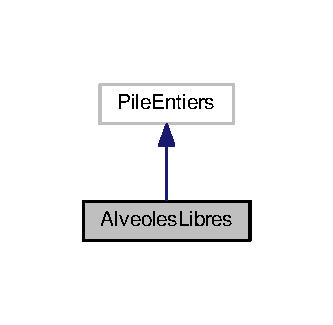
\includegraphics[width=160pt]{classAlveolesLibres__inherit__graph}
\end{center}
\end{figure}


Collaboration diagram for Alveoles\+Libres\+:
\nopagebreak
\begin{figure}[H]
\begin{center}
\leavevmode
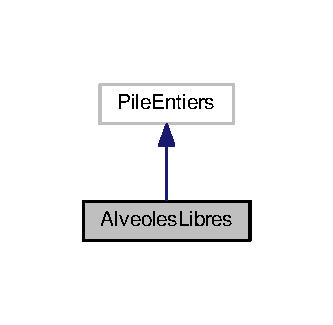
\includegraphics[width=160pt]{classAlveolesLibres__coll__graph}
\end{center}
\end{figure}
\subsection*{Public Member Functions}
\begin{DoxyCompactItemize}
\item 
\hyperlink{classAlveolesLibres_a66bc2220fd2c7b34cdc29d365cecc2d8}{Alveoles\+Libres} (const int \+\_\+nb\+Rangees=10, const int \+\_\+nb\+Colonnes=20)
\begin{DoxyCompactList}\small\item\em \hyperlink{classAlveolesLibres_a66bc2220fd2c7b34cdc29d365cecc2d8}{Alveoles\+Libres\+::\+Alveoles\+Libres}. \end{DoxyCompactList}\item 
bool \hyperlink{classAlveolesLibres_abfc3b2d308004424b8414f80b7018ee5}{Reserver} (int \&\+\_\+rangee, int \&colonne)
\begin{DoxyCompactList}\small\item\em \hyperlink{classAlveolesLibres_abfc3b2d308004424b8414f80b7018ee5}{Alveoles\+Libres\+::\+Reserver}. \end{DoxyCompactList}\item 
void \hyperlink{classAlveolesLibres_a29b8a616b49c095bb6a6eefddc938c30}{Liberer} (const int \+\_\+rangee, const int \+\_\+colonne)
\begin{DoxyCompactList}\small\item\em \hyperlink{classAlveolesLibres_a29b8a616b49c095bb6a6eefddc938c30}{Alveoles\+Libres\+::\+Liberer}. \end{DoxyCompactList}\end{DoxyCompactItemize}


\subsection{Constructor \& Destructor Documentation}
\index{Alveoles\+Libres@{Alveoles\+Libres}!Alveoles\+Libres@{Alveoles\+Libres}}
\index{Alveoles\+Libres@{Alveoles\+Libres}!Alveoles\+Libres@{Alveoles\+Libres}}
\subsubsection[{\texorpdfstring{Alveoles\+Libres(const int \+\_\+nb\+Rangees=10, const int \+\_\+nb\+Colonnes=20)}{AlveolesLibres(const int _nbRangees=10, const int _nbColonnes=20)}}]{\setlength{\rightskip}{0pt plus 5cm}Alveoles\+Libres\+::\+Alveoles\+Libres (
\begin{DoxyParamCaption}
\item[{const int}]{\+\_\+nb\+Rangees = {\ttfamily 10}, }
\item[{const int}]{\+\_\+nb\+Colonnes = {\ttfamily 20}}
\end{DoxyParamCaption}
)}\hypertarget{classAlveolesLibres_a66bc2220fd2c7b34cdc29d365cecc2d8}{}\label{classAlveolesLibres_a66bc2220fd2c7b34cdc29d365cecc2d8}


\hyperlink{classAlveolesLibres_a66bc2220fd2c7b34cdc29d365cecc2d8}{Alveoles\+Libres\+::\+Alveoles\+Libres}. 


\begin{DoxyParams}{Parameters}
{\em \+\_\+nb\+Rangees} & \\
\hline
{\em \+\_\+nb\+Colonnes} & \\
\hline
\end{DoxyParams}
Constructeur de la classe alveoles\+Libres, initialise le nombre de rangées et de colonnes disponibles. 

\subsection{Member Function Documentation}
\index{Alveoles\+Libres@{Alveoles\+Libres}!Liberer@{Liberer}}
\index{Liberer@{Liberer}!Alveoles\+Libres@{Alveoles\+Libres}}
\subsubsection[{\texorpdfstring{Liberer(const int \+\_\+rangee, const int \+\_\+colonne)}{Liberer(const int _rangee, const int _colonne)}}]{\setlength{\rightskip}{0pt plus 5cm}void Alveoles\+Libres\+::\+Liberer (
\begin{DoxyParamCaption}
\item[{const int}]{\+\_\+rangee, }
\item[{const int}]{\+\_\+colonne}
\end{DoxyParamCaption}
)}\hypertarget{classAlveolesLibres_a29b8a616b49c095bb6a6eefddc938c30}{}\label{classAlveolesLibres_a29b8a616b49c095bb6a6eefddc938c30}


\hyperlink{classAlveolesLibres_a29b8a616b49c095bb6a6eefddc938c30}{Alveoles\+Libres\+::\+Liberer}. 


\begin{DoxyParams}{Parameters}
{\em \+\_\+rangee} & n° de la rangée de l\textquotesingle{}alvéole à libérer \\
\hline
{\em \+\_\+colonne} & n° de la colonne de l\textquotesingle{}alvéole à libérer\\
\hline
\end{DoxyParams}
Ajoute l’alvéole dont les coordonnées sont passées en paramètre à l\textquotesingle{}ensemble des alvéoles libres. \index{Alveoles\+Libres@{Alveoles\+Libres}!Reserver@{Reserver}}
\index{Reserver@{Reserver}!Alveoles\+Libres@{Alveoles\+Libres}}
\subsubsection[{\texorpdfstring{Reserver(int \&\+\_\+rangee, int \&colonne)}{Reserver(int &_rangee, int &colonne)}}]{\setlength{\rightskip}{0pt plus 5cm}bool Alveoles\+Libres\+::\+Reserver (
\begin{DoxyParamCaption}
\item[{int \&}]{\+\_\+rangee, }
\item[{int \&}]{\+\_\+colonne}
\end{DoxyParamCaption}
)}\hypertarget{classAlveolesLibres_abfc3b2d308004424b8414f80b7018ee5}{}\label{classAlveolesLibres_abfc3b2d308004424b8414f80b7018ee5}


\hyperlink{classAlveolesLibres_abfc3b2d308004424b8414f80b7018ee5}{Alveoles\+Libres\+::\+Reserver}. 


\begin{DoxyParams}{Parameters}
{\em \+\_\+rangee} & \\
\hline
{\em colonne} & \\
\hline
\end{DoxyParams}
\begin{DoxyReturn}{Returns}
vrai si une alvéole libre, faux si aucune alvéole n’est disponible
\end{DoxyReturn}
Fournit la localisation de l\textquotesingle{}alvéole (sa rangée et sa colonne). Elle la supprime également des alvéoles libres. 

The documentation for this class was generated from the following files\+:\begin{DoxyCompactItemize}
\item 
alveoleslibres.\+h\item 
alveoleslibres.\+cpp\end{DoxyCompactItemize}

\hypertarget{classAlveolesWidget}{}\section{Alveoles\+Widget Class Reference}
\label{classAlveolesWidget}\index{Alveoles\+Widget@{Alveoles\+Widget}}


Inheritance diagram for Alveoles\+Widget\+:
\nopagebreak
\begin{figure}[H]
\begin{center}
\leavevmode
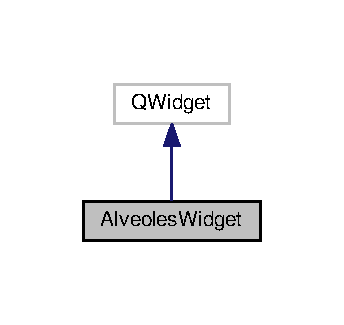
\includegraphics[width=165pt]{classAlveolesWidget__inherit__graph}
\end{center}
\end{figure}


Collaboration diagram for Alveoles\+Widget\+:
\nopagebreak
\begin{figure}[H]
\begin{center}
\leavevmode
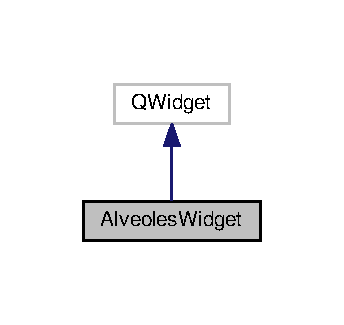
\includegraphics[width=165pt]{classAlveolesWidget__coll__graph}
\end{center}
\end{figure}
\subsection*{Public Member Functions}
\begin{DoxyCompactItemize}
\item 
{\bfseries Alveoles\+Widget} (Q\+Widget $\ast$parent=nullptr)\hypertarget{classAlveolesWidget_a1f0023fc1fc22fcdaae62d740f9f63c7}{}\label{classAlveolesWidget_a1f0023fc1fc22fcdaae62d740f9f63c7}

\end{DoxyCompactItemize}


The documentation for this class was generated from the following files\+:\begin{DoxyCompactItemize}
\item 
alveoleswidget.\+h\item 
alveoleswidget.\+cpp\end{DoxyCompactItemize}

%--- End generated contents ---

% Index
\backmatter
\newpage
\phantomsection
\clearemptydoublepage
\addcontentsline{toc}{chapter}{Index}
\printindex

\end{document}
